\chapter{Coordinates}
\index{Coordinates|textbf}

%-----------------------------------------------------------------------------
\section{Reference Orbit}
\label{s:ref}
\index{Coordinates!reference orbit|textbf}

The \vn{reference orbit} is the curved path used to define a coordinate
system for particles as shown in Figure~\ref{f:local_coords}.  At a
given time $t$, a particle's position can be described by a point on
the reference orbit a distance $s$ relative to the reference orbit's
zero position plus a transverse offset. This point on the reference
orbit is used as the origin of the local $(x, y, z)$ coordinate system
with the $z$--axis tangent to the reference orbit and pointing in the
direction of increasing $s$. The $x$ and $y$--axes are
perpendicular to the reference orbit. If the lattice has no vertical
bends, the $y$--axis is in the vertical direction and the $x$--axis is
in the horizontal plane. Notice that by construction, the particle is
always at $z = 0$.

\begin{figure}[tb]
\centering
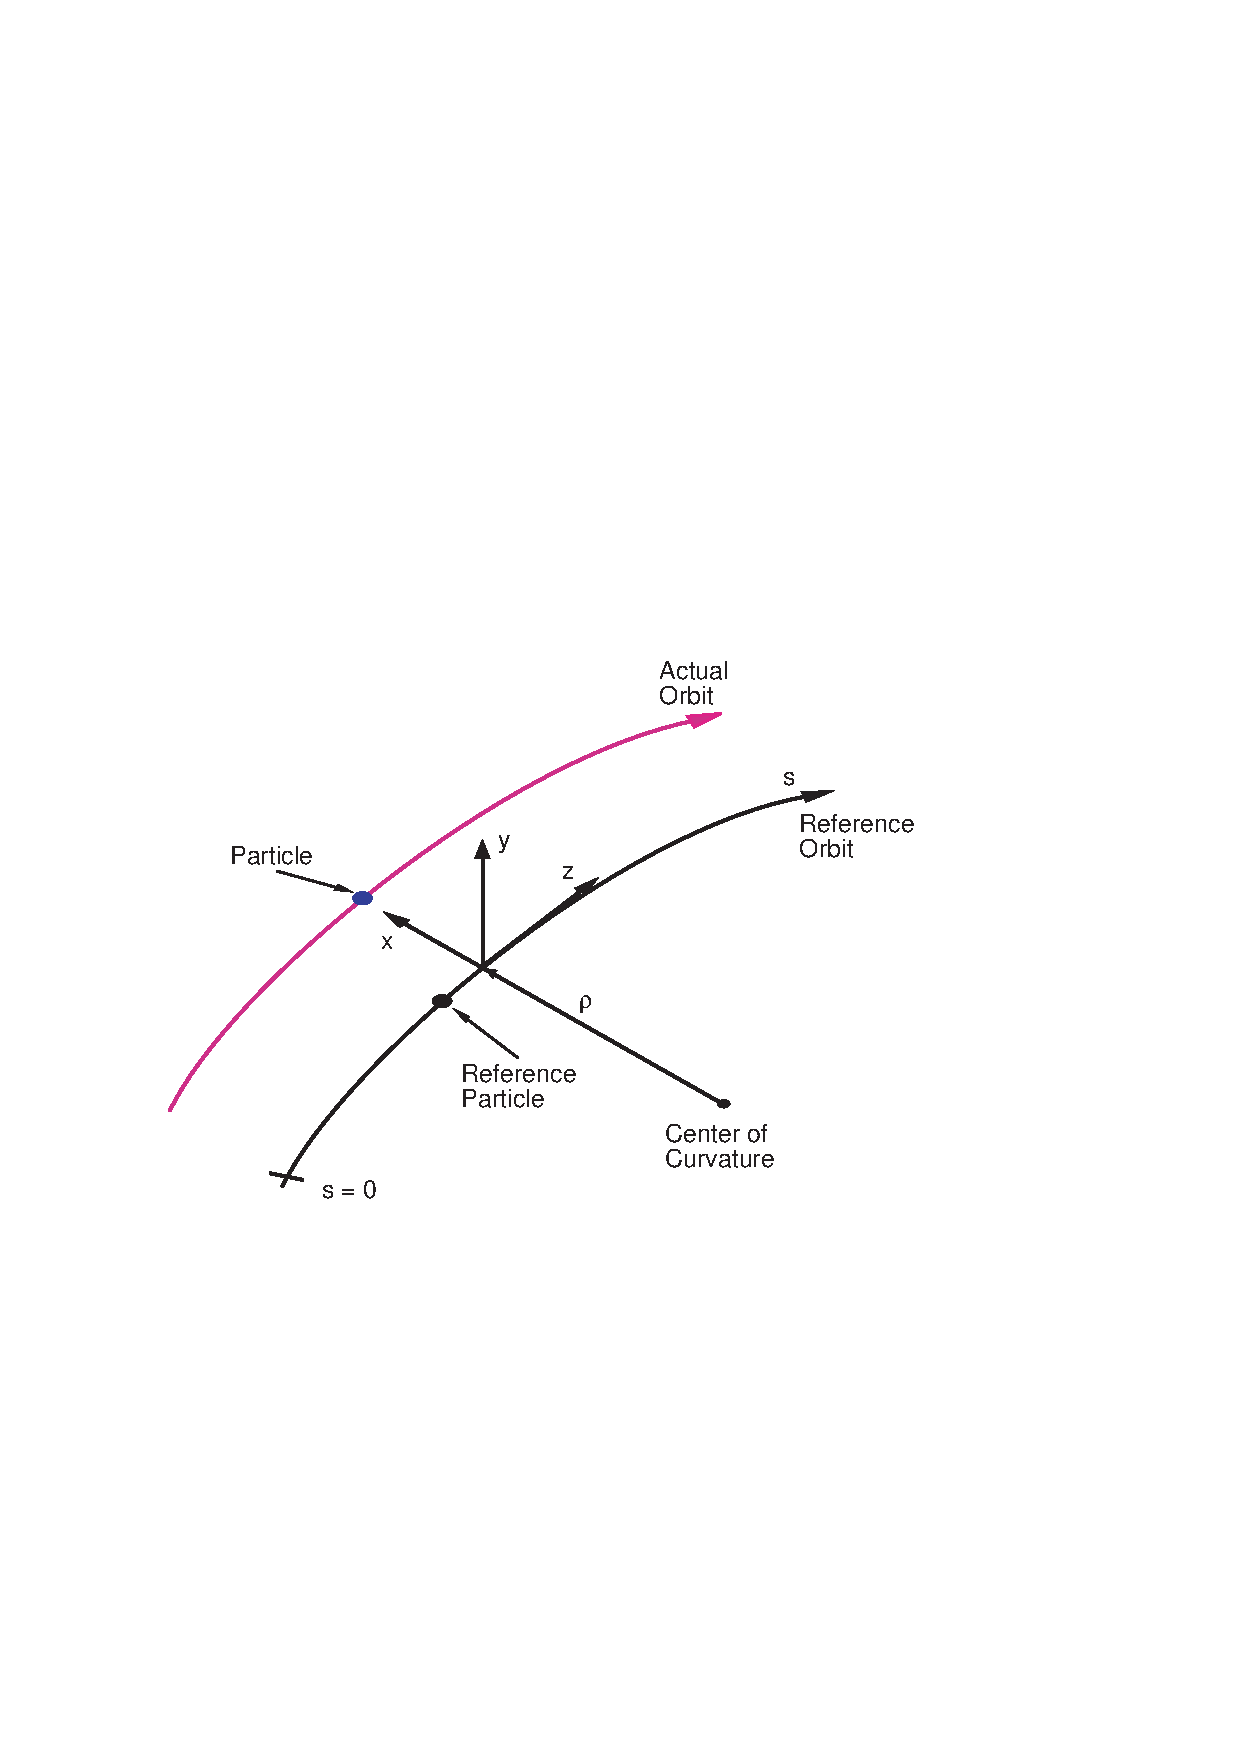
\includegraphics{local_coords.psfig}
\caption[The Local Reference System.]
{The Local Reference System. By construction, $z = 0$ for
the particle coordinates in the local reference system.}
\label{f:local_coords}
\end{figure}

\index{Sbend}
\index{Rbend}
\index{Element!entrance end}
\index{Element!exit end}
\index{Patch}
In \bmad, a lattice is comprised of a sequence of elements such as
quadrupoles, bends, RF cavities, etc. Each element has an entrance
point, an exit point, and a reference curve between them. For a bend,
the reference curve is a segment of a circular arc. For all other
elements, the reference curve is a straight line segment. The
reference orbit itself is constructed by arranging the elements so
that the exit point of one element coincides with the entrance point
of the next with the reference curves forming an arc with no kinks.
The reference orbit is then the sum of the reference
curves. Exceptions to this construction method may be made by using
\vn{Patch} elements which can arbitrarily offset the entrance point
of an element with respect to the exit point of the previous element.
See Section~\ref{s:patch}.  If not specified otherwise, the $s = 0$
position is the entrance point of the first element.

\index{X_offset}
\index{Y_offset}
\index{X_pitch}
\index{Y_pitch}
\index{Wiggler}
Notice that, in a \vn{Wiggler}, the reference orbit, which is a
straight line, does {\em not} correspond to the orbit that any actual
particle could travel. Typically the physical entity of an element is
centered about the reference curve. However, by specifying offsets and
pitches (See \sref{s:offset}), the physical element may be
arbitrarily offset with respect to its reference curve.  Shifting a
physical magnet with respect to its reference curve generally means
that the reference curve does {\em not} correspond to the orbit that
any actual particle could travel.

Do not confuse this reference orbit (which defines the local
coordinate system) with the reference orbit about which the transfer
maps are calculated (\sref{s:twiss}). The former is fixed by the
lattice while the latter can be any arbitrary orbit.

%-----------------------------------------------------------------------------
\section{Global Reference System}
\label{s:global}
\index{Coordinates!global|textbf}

The global reference system describes the orientation of the reference
orbit with respect to the laboratory coordinate system.  \bmad,
following the \mad\ convention, uses a Cartesian coordinate system
$(X, Y, Z)$ for the global reference system, along with three angles
$\theta, \phi, \psi$ used to define the reference orbit's orientation
as shown in Figure~\ref{f:global_coords}. Conventionally, $Y$ is the
vertical coordinate and $(X, Z)$ are the ``floor'' coordinates.  The
three angles are defined as follows:
\begin{description}
\item[$\theta$ Azimuth angle:] Angle in the $(X, Z)$ plane 
between the $Z$--axis and the projection of the $z$--axis onto the
$(X, Z)$ plane. A positive angle of $\theta = \pi/2$ corresponds to the
projected $z$--axis pointing in the positive $X$ direction.
\item[$\phi$ Pitch (elevation) angle:] Angle between the $z$--axis 
and the $(X,Z)$ plane. A positive angle of $\phi = \pi/2$ corresponds to
the $z$--axis pointing in the positive $Y$ direction.
\item[$\psi$ Roll angle:] Angle of the $x$--axis with respect 
to the line formed by the
intersection of the $(X, Z)$ plane with the $(x, y)$ plane. A
positive $\psi$ forms a right--handed screw with the $z$--axis.
\end{description}

\begin{figure}
\centering
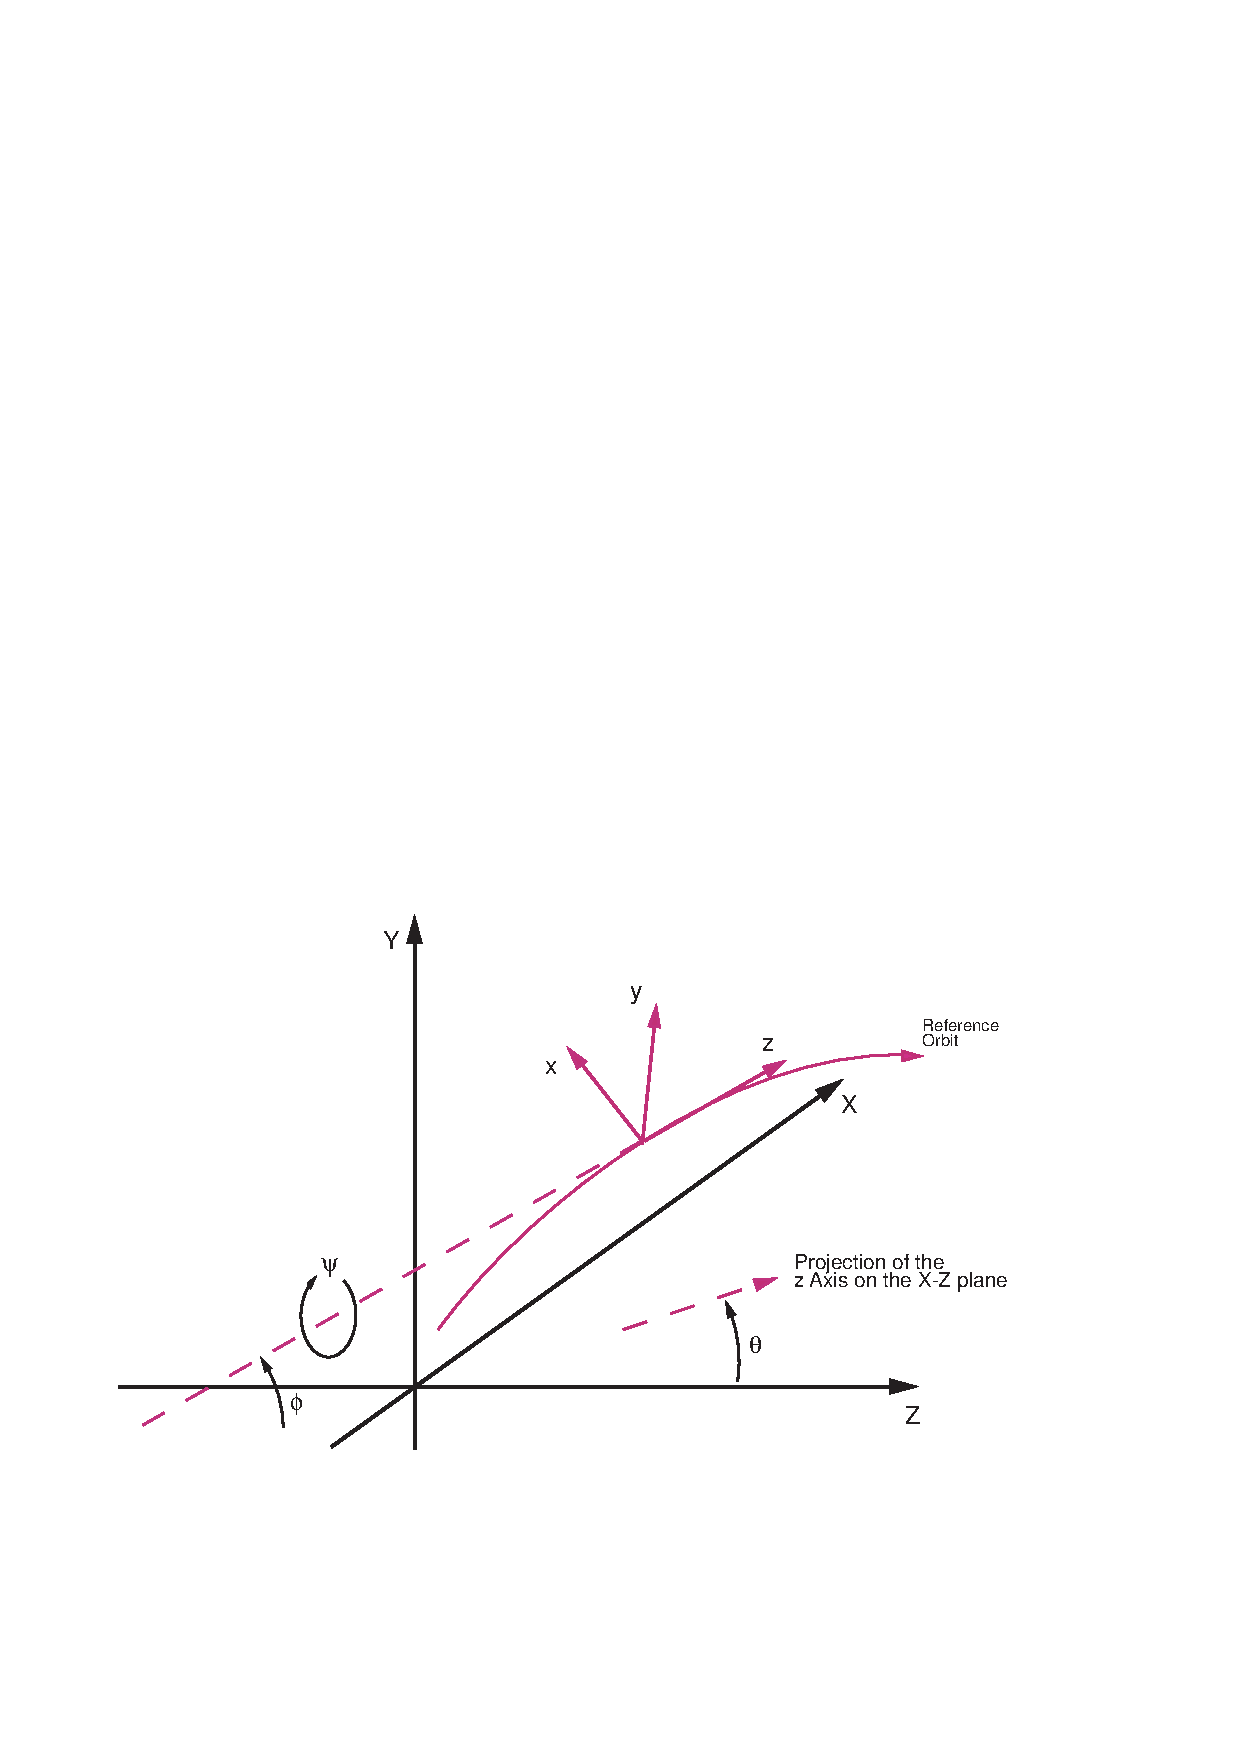
\includegraphics{global_coords.psfig}
\caption{The Global Reference System}
\label{f:global_coords}
\end{figure}

\index{Beginning statement}
\index{Coordinates!reference orbit!origin in global coordinates}
By default, at $s = 0$, the reference orbit's origin coincides with
the $(X, Y, Z)$ origin and the $x$, $y$, and $z$ axes correspond to
the $X$, $Y$, and $Z$ axes respectively. $\theta$ decreases as one
follows the reference orbit when going through a horizontal bend with
a positive bending angle. This corresponds to $x$ pointing radially
outward. Without any vertical bends, the $Y$ and $y$ axes will
coincide, and $\phi$ and $\psi$ will both be zero. The \vn{beginning}
statement (\sref{s:beginning}) in a lattice file can be use to override
this default.

\vfill

%-----------------------------------------------------------------------------
\section{Phase Space Coordinate System}
\label{s:phase_space_coords}
\index{Coordinates!phase space|textbf}

\bmad uses the canonical phase space coordinates 
\Begineq
  \Bf r(s) = (x, p_x, y, p_y, z, p_z)
\Endeq
The longitudinal position $s$ is the independent variable instead of
the time.  $x$ and $y$, are the reference orbit coordinates given in
Section~\ref{s:ref}.  The canonical momenta $p_x$ and $p_y$ are
normalized momenta
\begin{align}
  p_x = &\frac{P_x}{P_0} \\
  p_y = &\frac{P_y}{P_0}
\end{align}
where $P_x$ and $P_y$ are respectively the momentum components along
the $x$ and $y$ axes, and $P_0$ is the reference (sometimes called the
design) momentum.

The canonical $z$ coordinate is 
\Begineq
  z(s) = s - \beta \, c \, t 
\Endeq
where $t$ is the time at which the particle is at
position $s$, and $\beta = v/c$ with $v(s)$ being the velocity at position $s$. 
Do not confuse the canonical $z$ with the particle's longitudinal coordinate
in the local reference frame $z$ which is always zero as shown in
Figure~\ref{f:local_coords}.

A physical interpretation of canonical $z$ is given by
imagining a reference particle travelling along the reference curve who arrives
at position $s$ at time $t_0 = s / \beta c$. $z$ is then given by
\begin{align}
  z &= -\beta \, c \, (t - t_0) \CRNO
    &\equiv - \beta \, c \, \Delta t
\end{align}
$\Delta t$ being the time difference between when the
particle passes by a given $s$ position along the reference orbit and
when the reference particle does. $z$ is then the longitudinal distance
between the particle and the reference particle when the particle is at $s$
with positive $z$ indicating that the particle is ahead of the reference 
particle. At constant velocity $z$ can also be interpreted as the 
path length difference between the
particle as it passes a given $s$ position relative to the
path length of the reference particle as it passes the same $s$
position. 

The longitudinal canonical momentum $p_z$ is given by
\begin{equation}
  p_z = \frac{\Delta P}{P_0} \equiv \frac{P - P_0}{P_0}
\end{equation}
where $P$ is the momentum of the particle. For ultra--relativistic particles
$p_z$ can be approximated by
\begin{equation}
  p_z = \frac{\Delta E}{E_0}
\end{equation}
where $E_0$ is the reference energy (energy here always refers to the
total energy) and $\Delta E = E - E_0$ is the deviation of the
particle's energy from the reference energy. 

\index{Coordinates!phase space!MAD convention}
\index{MAD!phase space convention}
\mad uses a slightly different coordinate system where $(z, p_z)$ is
replaced by $(-c\Delta t, p_t)$ where $p_t \equiv \Delta E / P_0
c$. For highly relativistic particles the two coordinate systems are
identical.

\bmad generally uses the small angle (paraxial) approximation
where it is assumed that $p_x, p_y \ll 1$. With this approximation, the
relationship, between the canonical momenta and the slopes $x' \equiv dx/ds$
and $y' \equiv dy/ds$ is
\begin{align}
  x' &\approx \frac{p_x - a_x}{1 + p_z} (1 + g x) \\
  y' &\approx \frac{p_y - a_y}{1 + p_z} (1 + g x) 
\end{align}
$\Bf a = q \, A / c \, P_0$ is the normalized vector potential, $g =
1/\rho$ is the curvature function with $\rho$ being the radius of
curvature of the reference orbit and it has been assumed that the
bending is in the $x$--$z$ plane. 

\index{Coordinates!phase space!PTC convention}
\index{FPP/PTC!phase space convention}
For those programmers using the PTC\index{PTC/FPP}
software package directly (ignore
this if you don't know what I'm talking about) \'Etienne Forest uses,
by default, a different coordinate system where $(z, p_z)$ is replaced
by $(p_z, -z)$. However, PTC also has the ability to switch to the
coordinate system $(p_t, c \Delta t)$.